\chapter{Executive Summary}
\label{ch:intro}


%%%%%%%%%%%%%%%%%%%%%%%%%%%%
\section{The DUNE Near Detector Science Program}
\label{intro:science}
%\fixme{I like this title better than just ``Physics''}
The primary goal of the \dword{dune} 
\dword{nd} is to perform critical measurements near the \dword{lbnf} neutrino beam prior to the onset of neutrino oscillation effects to minimize the systematic uncertainties in  the long baseline neutrino oscillation measurements. Data from the \dword{nd} provides information on the neutrino flux, %their interaction 
the neutrino interactions on argon nuclei, and the response of the detector to the particles that emerge from the interaction necessary to accurately predict the observed spectrum of each neutrino species at the \dword{fd}
in the presence of neutrino oscillations and backgrounds. The \dword{lbl} %long baseline 
neutrino oscillation measurement is in effect an integrated measurement between \dword{nd} and \dword{fd}, where the \dword{fd} spectrum predicted using data from \dword{nd} as a function of the neutrino oscillation parameters is compared to the observations at \dword{fd} to extract the neutrino oscillation parameters. To this end, the \dword{nd} must provide sufficient information through its measurements to minimize the systematic uncertainties in the \dword{fd} which would otherwise suffer large uncertainties if otherwise unconstrained predictions based on {\em ab initio} simulations are used.

The requirements and design of \dword{nd} are driven by the needs of the \dword{lbl} %long baseline 
neutrino oscillation measurements, and therefore are tightly coupled to the  expected measurement capabilities and systematic uncertainties at the \dword{fd}.

Except where explicitly noted, we assume that any discussion of neutrinos also refers to antineutrinos, including data-taking with \dword{lbnf} in both neutrino-enhanced forward horn current (FHC) and antineutrino-enahced (RHC) modes.

%%%%%%%%%%%%%%
\subsection{Other Physics}
\label{intro:science:other}
The intense neutrino beam produced by \dword{lbnf} can support a wide range of physics measurements and studies using \dword{nd}, including:
\begin{itemize}
    \item {\bf Neutrino-nucleus interactions studies:} A large variety of interactions can be studied due to the reconstruction capabilities of the detector, the wide energy range, assortment of materials and nuclear targets with high statistics. 
    \item {\bf Short baseline neutrino oscillations:} Exotic neutrino states with large mass splittings may induce neutrino oscillations on a short distance scale which may be visible in the \dword{nd} %near detector 
    system.
    \item {\bf Exotic physics  :} The \dword{lbnf} neutrino beam may produce exotic particles in the primary proton interactions on the target, the subsequent decay of secondary particles, or through neutrino interactions which may be detectable through their interaction or decay in the near detector system.
\end{itemize}
Neutrino-nucleus interaction studies at \dword{nd}, particularly on argon, are intimately connected to its primary role in the long baseline neutrino oscillation program, but differ in providing independent measurements on the property of these interactions rather than integrating them into the extraction of neutrino oscillation parameters. Due to this difference, the channels of interest and measurement strategy may differ considerably between in the two cases. Neutrino-nucleus interaction measurements also support other DUNE physics goals, such as the search for nucleon decay in the \dword{fd} or exotic particle searches in either detector, where they may improve the estimate of backgrounds arising from neutrino interactions.

The requirements of these additional physics programs do not explicitly drive the design of \dword{nd} but the extensive capabilities needed to deliver the requirements for the long baseline measurements will enable a compelling program in these other areas.

%%%%%%%%%%%%%%
\subsection{Neutrino Oscillations}
\label{intro:science:nuosc}
%Relatively standard introduction . . .  follow TDR/ND CDR
The quantum mechanical mixing of neutrino flavor and mass states which manifests in a time dependence to the flavor content of a neutrino, called neutrino oscillations. Since neutrinos are typically produced and interact in flavor states via the weak interaction, this mixing allows the possibility that a neutrino is produced in one flavor and interacts in a different flavor. This probability oscillates as a function of $L/E$, where $L$ is the distance between the production and interaction of the neutrino and $E$ is its energy. The frequency of these oscillations in $L/E$ are set by the differences squared mass eigenvalues ($\Delta m_{ij}^2$) and the amplitudes by the mixing matrix $U_{ij}$ which relates the mass and flavor eigenstates of the neutrino.
\begin{itemize}
    \item 
\item $P(\nu_\mu\to\nu_e)$
\end{itemize}
.  ,  governed by the unitary mixing matrix relating the flavor and mass states and the mass splittings, 


%%%%%%%%%%%%%%
\subsection{Goals of Experiment}
\label{intro:science:goals}
Neutrino oscillations are measured by comparing the observed spectrum of the neutrino interactions observed at the \dword{fd} to the predicted spectrum, which results from a convolution over neutrino energy ($E_\nu$) of the following quantities:
\begin{itemize}
    \item $\Phi_\alpha(E_\nu)$: The initial flux and spectrum produced by the \dword{lbnf} beam in each flavor $\nu_\alpha$.
    \item $P(\nu_\alpha\to\nu_\beta,E_\nu)$: The probability for oscillation from the initial flavor $\nu_\alpha$ to the flavor $\nu_\beta$ due to neutrino oscillations, determined by the neutrino mass and mixing parameters.
    \item $\sigma_\beta(E_\nu)$: The modeling of the $\nu_\beta$ with energy $(E_\nu)$ on the argon nucleus including its interaction cross section and resulting outgoing particles.
%    \item $V\times n$: The number of argon target nuclei in the \dword{fd}
    \item $R_\beta(E_\nu)$:  The response of the detector to the interaction of $\nu_\beta$ to produce observables to select and kinematically characterize ({\em e.g.} reconstruct the neutrino energy) of a $\nu_\beta$ interaction. 
\end{itemize}
Assuming the $\Phi_\alpha$, $\sigma_\beta$, and $R_\beta$ are well-understood, the oscillation parameters governing $P(\nu_\alpha\to\nu_\beta)$ can be extracted. Figure \ref{fig:fd_nmu_nue}

Background
%Long baseline neutrino physics
%Emphasize multiparameter nature of the physics . . . . it’s not just about nue appearance, but in order to extract %parameters, including CPV correctly, DUNE must also be able to extract theta23, Dm2, etc. correctly.  Otherwise, DUNE’s %own measurements will either be in tension or biased.
%Explain the timeline for neutrino oscillation measurements .. . when do we expect to achieve certain milestones in %sensitivity/precision in order to set up staging discussion later.

\begin{dunefigure}[$\nu_\mu$,$\nu_e$ at \dword{fd}]{fig:fd_nmu_nue}
%  \centering
{Spectrum of $\nu_\mu$, $\nu_e$}
  \subfloat[][$E_{\rm rec}$]{
    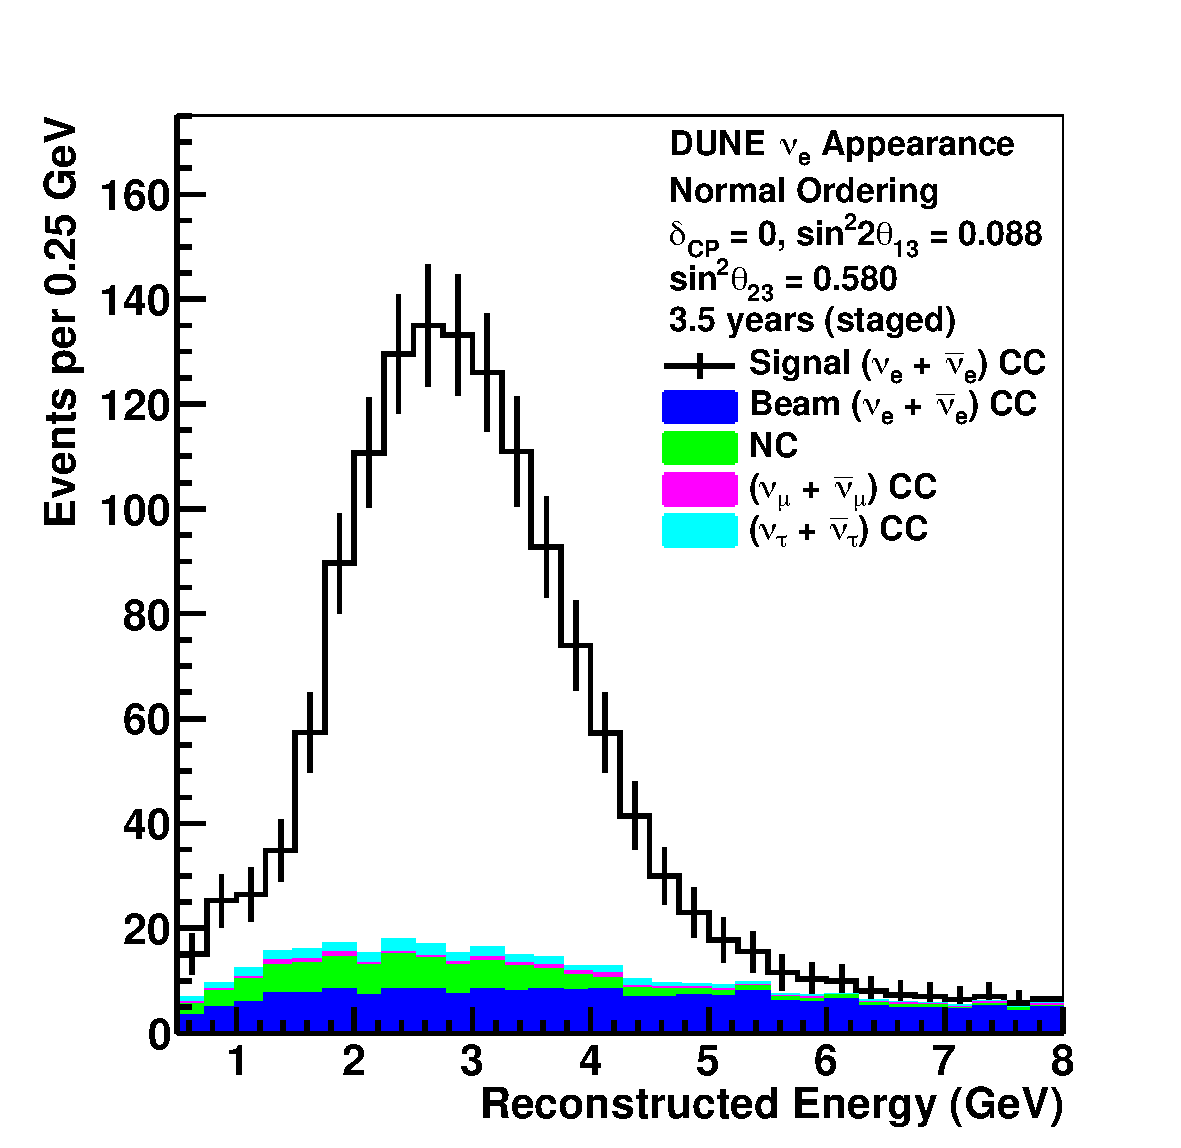
\includegraphics[width=0.45\textwidth]{spec_app_nu_no.pdf}

    %\label{fig:fd_nue}
  }
  \subfloat[][$E_{\rm proton}^{dep}$]{
    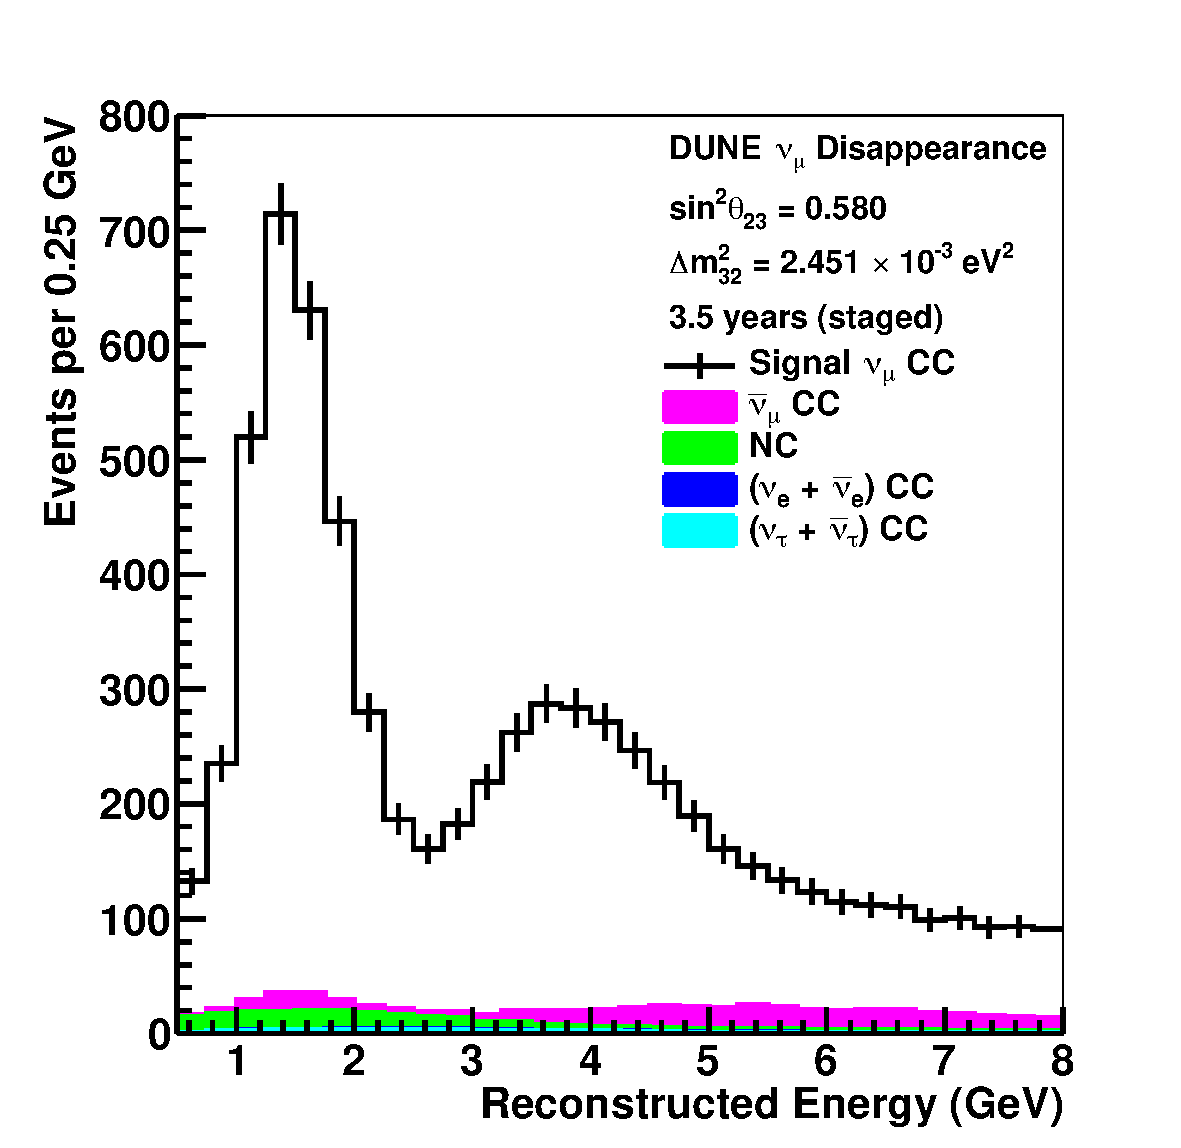
\includegraphics[width=0.45\linewidth]{spec_dis_nu_no.pdf}
    %\label{fig:fd_numu}
  }
\end{dunefigure}


%%%%%%%%%%%%%%
\subsection{Role of Near Detector}
\label{intro:science:role}


The role of the \dword{nd} in the long baseline neutrino oscillation analysis is summarized within the \dword{dune} Global Science Requirements:

{\em \dword{nd} measurements shall be of sufficient precision to ensure that when extrapolated to \dword{fd} to predict the \dword{fd} event spectra, the associated systematic error must not dominate the measurement precision.''}

To that end, the \dword{nd} must:
\begin{itemize}
    \item make measurements to constrain uncertainties in each component of the \dword{fd} prediction mentioned above, namely the initial neutrino fluxes $\phi_\alpha$, the neutrino interaction modeling $\sigma_\beta$, and the detector response $R_\beta$, so that in their total impact in predicting the \dword{fd} event spectra is less than the statistical uncertainty in the \dword{fd}. 
    \item have measurement capabilities sufficiently robust to mitigate unexpected sources of uncertainty in any part of the prediction. 
\end{itemize}

We summarize several key challenges which drive the requirements for \dword{nd} to fulfill these roles.

\subsection{Initial Neutrino Flux $\Phi_\alpha$:}
Over the past few decades, significant progress has been made in predicting the neutrino flux resulting from high-energy proton-based neutrino beam lines such as \dword{lbnf}. Several key elements in the prediction include:
\begin{itemize}
\item Detailed and precise modelling of the as-built neutrino beam line for simulation. This includes the geometry, material, and magnetic fields.
\item Measurements and monitoring of the primary proton beam optics .
\item Precise data on hadron production for the primary proton interactions on the target and secondary interactions both on the target and elsewhere (horn, {\em etc.}).
\item Secondary monitoring using muons penetrating the beam absorber to measure their lateral profile. 
\item Simulation incorporating all the above aspects.
\end{itemize}
Advances in these elements have resulted in  {\em ab initio} predictions of the neutrino flux from similar beam lines ({\em e.g.}\dword{t2k}, \dword{numi}) with uncertainties at the $\mathcal{O}(10\%)$ level or better. In contrast, previously, such predictions were considered inherently unreliable beyond a rough estimate. In particular hadron production measurements using replica targets have reduced the uncertainties in the prediction from hadron production to the level where other uncertainties (component alignment, secondary interactions, {\em etc.}) are comparable in size. 

The complexities and harsh operating conditions for neutrino beam lines result in the potential for unexpected deviations of the beam line from its nominal or as-built configuration and condition. This can result in significant variations and uncertainties in the neutrino flux if they are not identified and understood. In the most severe cases (electrical faults in the horn system, target failure, {\em etc.}), such deviations may cause the beam to be inoperable. Recent experience could be:
\begin{itemize}
    \item Target and other component degradation: The extreme thermal, shock, and radiation exposure of the target can result in target degradation, changing the both rate and distribution of the primary particle production and subsequent secondary in such a way that the hadron production off the target is different than expected.
    \item Component movement: The neutrino beam line serves as a precisely aligned focusing system for hadrons produced in the target. Movement of components relative to each other disturb the optics and change the focusing properties. Such changes can move the effective pointing direction of the beam or focus different parts of the hadron phase space and more generally changing the expected neutrino flux. 
\end{itemize}
In general, the high radiation environment make explicit checks of beam line components during operation limited and difficult, if not impossible. At best, they may require a prolonged interruption in the beam operation which would normally reserved for long term maintenance cycles like summer shutdowns. Monitoring on short time scales ({\em e.g.} pulse-by-pulse) can be performed by secondary beam monitors such as muon monitors downstream of the hadron absorber, but are limited. Verification of the nominal neutrino flux through ``standard candles'' of neutrino interactions and monitoring its time dependence through high-statistics inclusive channels is required. Explicit measurement of the neutrino flux and its stability are thus an essential role for \dword{nd}. 

Something about $\Phi_{FD}/\Phi_{ND}$

\begin{dunefigure}[$\nu_\mu$,$\nu_e$ at \dword{nd}]{fig:eproton_study}
%  \centering
{Spectrum of $\nu_\mu$, $\nu_e$}
  \subfloat[][$E_{\rm rec}$]{
    \includegraphics[width=0.45\textwidth]{hist_stop0_Erec_osc_noRW.png}

    %\label{fig:eproton_ndspec}
  }
  \subfloat[][$E_{res}$]{
    \includegraphics[width=0.45\linewidth]{FHC_Enu_Erec_fracDiff1D_m20pcProtonE.png}
    %\label{fig:eproton_enures}
  }
\end{dunefigure}





\begin{dunefigure}[$\nu_\mu$,$\nu_e$ at \dword{nd}]{fig:nuwro_study}
%  \centering
{Spectrum of $\nu_\mu$, $\nu_e$}
  \subfloat[][$Q^2$]{
    \includegraphics[width=0.45\textwidth]{graphics/PiStudyDataMCRatioTrueFHC.pdf}
    %\label{fig:eproton_ndspec}
  }
  \subfloat[][$\delta_{CP}$ ]{
    \includegraphics[width=0.45\linewidth]{graphics/PiStudyBiasWithGAr.pdf}
    %\label{fig:eproton_enures}
  }
\end{dunefigure}

\subsection{Neutrino Interaction Modelling $\sigma_\beta$:}
All the properties of an interacting neutrino must be inferred from its outgoing particles. As a result, the modelling of neutrino-nucleus ($\nu-A$) interactions, particularly on argon in the case of \dword{dune}, is a critical element of the analysis. Since the oscillation parameters are extracted from the energy spectrum of neutrino interactions in each flavor, the modelling must provide the interaction cross section, summarizing the likelihood that the neutrino of a given flavor and energy interacts at all, as well as the details of the outgoing lepton and hadron systems, which are essential ingredients in understanding metrics like efficiencies/purities of the selected events and the resolution of quantities like the neutrino energy. For the hadron system in particular, the details of the particle content (particle type and kinematics) fundamentally impact the ionization and optical signal of the events, and thus the detector response is sensitive to this modelling regardless of whether the event selection and kinematic reconstruction chooses to use the details of the information or not.
Likewise, the modelling issues go beyond the determination of the $\nu-A$ cross section, but in include all aspects of modelling the $\nu-A$ interaction and the particles emerging from the target nucleus that impact the detector response. To that end, reference to ``$\sigma_\beta$'' and ``neutrino cross sections'' encompasses these issues, and not just ``cross sections'' narrowly defined. However, we exclude particle tracking and propagation effects in bulk media ({\em e.g.} LAr) which also  

It has been widely recognized that as accelerator-based neutrino oscillation experiments have increased in precision, commensurate improvements in neutrino-nucleus interactions are necessary to limit their impact on the systematic uncertainty budget. While the past decade has seen substantial progress both in measurements and theoretical/modelling, significant challenges remain both in defining a ``default'' model and adequately quantifing and propagating systematic uncertainties.

Among the concerns and challenges include:
\begin{itemize}
\item A handful of well-developed neutrino event generators and other models for $\nu-A$ interactions are available to the community. However, the generators have significant differences in the predicted properties of the $\nu-A$ interactions, even when they employ similar underlying models.
\item There have been a few ``surprises'' in the form of significant deviations from model predictions resulting from physics processes that were not accounted for. One example is the excess of pionless $\nu_\mu$ charged current 
\item Theoretically, it is recognized that 

\end{itemize}

In each case
%Summary of Role of near detector in LBL physics
%Explain major a priori uncertainties in neutrino flux, neutrino interactions, detector response. Visit examples from NOvA %and T2K about how near detectors reduce uncertainties.
%Discussion on coupling/convolution of uncertainties.
%Discussion on “out-of-model” uncertainties with Genie/NuWRO and missing proton energy  examples as case studies. Past %experience and current state of knowledge suggests that such uncertainties are inevitable . . .  . we’re not dealing with %the Standard Model of particle physics.
%Figures: Reprise of standard plots (dCP/MO significance, theta23 precision). Bias in dCP from NuWRO/Genie study. Bias in %theta23, Dm2 from missing proton energy study.




%%%%%%%%%%%%%%%%%%%%%%%%%%%%
\section{The DUNE Collaboration and the DUNE-US Project}
\label{intro:collab-proj}

\fixme{You may want to change the title, but put the CDR-to-PDR-to-TDR explanation in this section along with some explanation of how it fits into the project}

%%%%%%%%%%%%%%%%%%%%%%%%%%%%
\section{Near Detector Reference Design}
\label{intro:refdes}
%Uncertainties (Flux, cross section, detector modelling)
%State overarching requirements, give rough sense of required overall systematic error.  
%Requirements
%List key measurements, purpose, and requirements.



%%%%%%%%%%%%%%
\subsection{PRISM}
\label{intro:refdes-prism}
%\fixme{I think it makes more sense to keep PRISM within the reference design rather than after it, no?}
%Quick overview of concept and applications, how to form pseudo-Gaussian beams, flux matching with oscillations. Reference %CDR for mathematical details.
%Plots: Pseudo-gaussian beam example, Flux matching example.



%%%%%%%%%%%%%%
\subsection{ND-LAr}
\label{intro:refdes-ndlar}

%%%%%%%%%%%%%%
\subsection{Cryostat}
\label{intro:refdes-cryostat}

%%%%%%%%%%%%%%
\subsection{TMS (or ND-Gar?)}
\label{intro:refdes-tms}





%%%%%%%%%%%%%%%%%%%%%%%%%%%%
\section{The LBNF Near Site Conventional Facilities}
\label{intro:lbnf}



%%%%%%%%%%%%%%%%%%%%%%%%%%%%
\section{Staging: The Day-One Detector}
\label{intro:staging}

%Revisit muon spectrometry requirements for ND-LAr interactions, sensitivity plots showing that first goals can be reached without ND-GAr.


%%%%%%%%%%%%%%%%%%%%%%%%%%%%
\section{The DUNE-US Project Organization and Responsibilities}
\label{intro:collab-proj}



%%%%%%%%%%%%%%%%%%%%%%%%%%%%
\section{Summary of DUNE-US Scope}
\label{intro:us-scope}
